% Tex root = ../cheatsheet.tex
\section{Differenzielle Analysis in R\textsuperscript{n}}
\subsection{Einleitung}
  \begin{itemize}
    \item[$*$] $[a,b]\rightarrow\mathbb R^m$ Pfad oder Weg
    \item[$*$] $\mathbb R^n\rightarrow\mathbb R$ Skalarfeld
    \item[$*$] $\mathbb R^n\rightarrow\mathbb R^n$ Vektorfeld
  \end{itemize}
\subsection{Stetigkeit}
  \definition{3.2.1}{Konvergenz einer Folge}
    Eine Folge $x_1,x_2,...\in\mathbb R^n$ konvergiert gegen $y\in\mathbb R^n$
    falls 
    $$
      \forall\varepsilon>0\;\exists N\forall k\geq N: ||x_k-y||<\varepsilon
    $$
    Dann schreibt man $\lim\limits_{i\rightarrow\infty}x_i=y$.\\
    $$\begin{array}{lclr}
      \lim\limits_{i\rightarrow\infty}x_i=y&\iff&\lim\limits_{i\rightarrow\infty}||x_i-y||=0&\\
      &\iff&\lim\limits_{i\rightarrow\infty}x_{i,j}=y\;\;\forall j\in\{1,...,n\}
    \end{array}$$
  \definition{3.2.3}{Stetigkeit}
    Eine Funktion $f:U\rightarrow \mathbb R^m$ auf $U\subseteq\mathbb R^n$
    heisst \textbf{stetig bei} $x_0\in U$ falls
    $\forall\varepsilon>0\exists\delta>0\forall x\in U:$
    $$||x-x_0||<\delta\implies||f(x)-f(x_0)||<\varepsilon$$
    und \textbf{stetig} falls $f$ bei jedem punkt $x_0\in U$ stetig ist.\\
  \proposition{3.2.4}{}
    $f$ stetig bei $x_0\iff$ Für jede Folge $x_0,x_1,...\in U$ mit
    $\lim\limits_{i\rightarrow\infty}x_i=x_0$ gilt
    $\lim\limits_{i\rightarrow\infty}f(x_i)=f(x_0)$\\
  \definition{3.2.5}{Konvergenz einer Funktion}
    $f:U\rightarrow\mathbb R^m$ konvergiert bei $x_0\in U$ gegeb $y\in\mathbb
    R^m$ falls $\forall\varepsilon>0\;\exists\delta>0\;\forall x\in U:$
    $$
      ||x-x_0||<\delta \text{ und } x\neq x_0\implies ||y-f(x)||<\varepsilon
    $$
    Dann schreibt man $\lim\limits_{\substack{x\rightarrow x_0\\x\neq x_0}}f(x)=y$.\\
  \proposition{3.2.7}{}
    $f: U\rightarrow V, g: V\rightarrow\mathbb W$ mit $U\subseteq\mathbb R^n$,
    $V\subseteq\mathbb R^m$ $f,g$ stetig $\implies g\circ f:U\rightarrow W$ ist
    stetig.\\\\
    $\lim\limits_{\substack{x\rightarrow x_0\\ x\neq x_0}}f(x)=y\iff$ Für jede
    Folge $x_1,x_2,...\in U\setminus\{x_0\}$ mit
    $\lim\limits_{i\rightarrow\infty} x_i=x_0$ gilt
    $\lim\limits_{i\rightarrow\infty}f(x_i)=y$\\
  \definition{3.2.11}{$U\subseteq\mathbb R^n$ heisst}
    \begin{enumerate}
      \item[$*$] \textbf{beschränkt} falls $\{||x||\mid x\in U\}\subseteq\mathbb
        R^+_0$
      \item[$*$] \textbf{abgeschlossen} falls $x_1,x_2,...\in U, 
        \lim\limits_{k\rightarrow\infty}x_k=y\in\mathbb R^n\implies y\in U$
      \item[$*$] \textbf{kompakt} falls $U$ beschränkt und abgeschlossen.
      \item[$*$] \textbf{offen} falls $\forall x\in U\;\exists\delta>0:$
        $$\{y\in\mathbb R^n\mid|x_i-y_i|<\delta\text{ für alle } i\}$$
    \end{enumerate}
  \proposition{3.2.13}{}
    $f:\mathbb R^n\rightarrow\mathbb R^m$ stetig. Dann:
    \begin{enumerate}
      \item[(1)] $V\subseteq\mathbb R^m$ abg $\implies 
        f^{-1}(V)\subseteq\mathbb R^n$ abg.
      \item[(2)] $V\subseteq\mathbb R^m$ offen $\implies
        f^{-1}(V)\subseteq\mathbb R^n$ offen.
    \end{enumerate}
  \proposition{3.2.15}{}
    $U\subseteq\mathbb R^n$ nicht-leer und kompakt, $f:U\rightarrow\mathbb R$
    stetig $\implies f$ nimmt auf $U$ $Min.$ und $Max.$ an, d.h. es gibt
    $x_+,x_-\in U$ sodass $\forall y\in U: f(x_-)\leq f(y)\leq f(x_+)$
\subsection{Parzielle Ableitungen}
  \proposition{3.3.2}{}
    $U\in\subseteq^n$ offen $\iff \mathbb R^n\setminus U$ abgeschlossen.\\
  \definition{3.3.5}{$i$-te partielle Ableitung}
    $U\subseteq\mathbb R^n$ offen, $f:U\rightarrow\mathbb R$. Für
    $i\in\{1,...,n\}$ ist die $i$-te partielle Ableitung von $f$ bei $y\in U$
    $$\partial_if(y)=g'(y_i)\in\mathbb R$$ für $g:\{t\in\mathbb
    R\mid(y_1,...,t,...,y_n))\in U\}\rightarrow\mathbb R$
    $$g(t)=f(y_1,...,t,...,y_n)$$ falls $g$ bei $y$ diffbar ist.\\
    \textbf{Weitere Schreibweisen:}\\
    $\partial_if=\partial_{x_i}f=f_{x_i}=\frac{\partial f}{\partial_{x_i}}$\\
  \definition{3.3.9}{Jacobimatrix}
    $U\subseteq\mathbb R^n$ offen, $f:U\rightarrow\mathbb R^m$. Die $m\times
    n$-Matrix $$J_f(x)=(\partial_jf_i(x))_{\substack{1\leq i\leq m\\1\leq j\leq
    n}}$$
    heisst Jacobimatrix von $f$ bei $x$.\\
\definition{3.3.11}{Gradient und Divergent}
  \textbf{Gradient}: Wenn für die Funktion $f:U\rightarrow \mathbb R$ alle partiellen Ableitungen existieren für $x_0\in U$, dann ist der Vektor $$\begin{pmatrix}\partial_{x_1}f(x_0)\\\vdots\\\partial_{x_n}f(x_0)\end{pmatrix}$$
    \textbf{Divergent} Wenn für eine Funktion $f=\{f_1,...,f_m\}:U\rightarrow\mathbb R^m$ alle partiellen ableitungen für alle $f_i$ bei $x_0\in U$ existieren, ist der Divergent die Trace der Jakobimatrix $$div(f)(x_0)=Tr(J_f(x_0))$$
\subsection{Das Differential}
\definition{3.4.2}{Differenzierbarkeit}
  Wenn \(U\in\mathbb R^n\) eine offene Menge, \(f:U\rightarrow R^m\) eine Funktion und $A: \mathbb R^n\rightarrow\mathbb R^m$ eine affine Abbildung ist, dann ist $f$ bei $x_0\in U$ differenzierbar mit Differenzial A, falls:
  \[\lim\limits_{\substack{x\rightarrow x_0 \\ x\neq x_0}}\frac{f(x)-f(x_0)-A(x-x_0)}{||x-x_0||}=0\]\\
\proposition{3.4.4}{Eigenschaften von differenzierbaren Funktionen}
  Wenn \(U\in\mathbb R^n\) eine offene Menge, \(f:U\rightarrow R^m\) eine differenzierbare Funktion dann gilt:
  \begin{enumerate}
    \item Die Funktion $f$ ist stetig auf $U$
    \item Für die Funktion $f=[f_1,...,f_m]$ existieren alle \(\partial_{x_j}f_i\) mit \(1\leq j \leq n, 1\leq i\leq m\)
  \end{enumerate}
\proposition{3.4.6}{Differenzierbarkeit bei Funktionsoperationen} 
  \(U\in\mathbb R^n\) offen, \(f,g:U\rightarrow\mathbb R^m\) differenzierbar:
  \begin{enumerate}
    \item \(f+g\) ist differenzierbar und \\ $d(f+g)(x_0)=df(x_0)+dg(x_0)$
    \item Falls \(m=1: f\cdot g\) differenzierbar.
    \item Falls \(m=1, g\neq0:\frac f g\) differenzierbar.
  \end{enumerate}
\proposition{3.4.7}{Differenzial von elementaren Funktionen}
\proposition{3.4.9}{Kettenregel} \(U\in\mathbb R^n\) und \(V\in\mathbb R^m\) offen, \(f:U\rightarrow V, g:V\rightarrow\mathbb R^p\) differenzierbar.\\
\textbf{Funktionen:} 
Dann ist $g\circ f$ differenzierbar und $d(g\circ f)(x_0)=dg(f(x_0))\circ df(x_0)$.\\
\textbf{Jakobi Matrizen:}
\(J_{g\circ f}(x_0)=J_g(f(x_0)\cdot J_f(x_0)\).\\
\textbf{Gradienten:}
\(\bigtriangledown_{g\circ f}=J{g\circ f}^T, \bigtriangledown_g=J_g^T\) also
\(\bigtriangledown_{g\circ f}(x_0)=J_f(x_0)^T\cdot\bigtriangledown_g(f(x_0))\).\\
\definition{3.4.11}{Der Tangentialraum}
  \(U\in\mathbb{R}^n\) offen, \(f: U\rightarrow\mathbb{R}^m\) differenzierbar, \(x_0\in U\), \(A=df(x_0)\). Der Tangentialraum bei \(x_0\) des Graphen von \(f\) ist der Graph von \(g(x)=f(x_0)+A(x-x_0)\), also \(T=\{(x,g(x))\mid x\in\mathbb{R}^n\}\subseteq\mathbb{R}^n\times\mathbb{R}^m\).\\
\definition{3.4.13}{Richtungsableitung}
  \(U\in\mathbb{R}^n\) offen, \(f:U\rightarrow \mathbb{R}^m, v\in\mathbb{R}^n\setminus\{0\}\), \(x_0\in U\). Die Richtungsableitung von \(f\) bei \(x_o\) in Richtung \(v\) ist \[D_v f(x_o) := J_g(0)=\begin{pmatrix}g'(0)_1\\\vdots\\g'(0)_m\end{pmatrix}\in\mathbb R^m\] für die Hilfsfunktion \(g : \{t\in\mathbb R\mid x_0 + tv\in U\}\rightarrow \mathbb R ^m\) \(g(t)=f(x_0+tv)\)\\
\proposition{3.4.15}{Richtungsableitung von differenzierbaren Funktionen Berechnen}
  \(U\in\mathbb R^n\) offen, \(f:U\rightarrow\mathbb R^m\) differenzierbar, \(v\in\mathbb R^m\setminus\{0\}, x_0\in U\). \\\(\implies D_vf(x_0)=df(x_0)(v)=J_f(x_0)\cdot v\) was auch bedeutet, dass die Richtungsableitung linear vom Richtungsvektor abhängen.\\
  \(\implies D_{\lambda_1v_1+\lambda_2v_2}=\lambda_1D_{v_1}f(x_0)+\lambda_2D_{v_2}f(x_0)\)\\
  \example{3.4.17}{Richtungsableitung von allgemeinen stetigen Funktionen berechnen.}
  \(D_vf(x_0)=\lim\limits_{t\rightarrow0}\frac{f(x_0+tv)-f(x_0)}{t}\) Sollte die
  daraus resultierende Funktion nicht linear von \(v\) abhängig sein, so ist
  \(f\) nicht differenzierbar.
\subsection{Höhere Ableitungen}
  \definition{3.5.1}{C Notation}
    \(U\subseteq\mathbb R^n\) offen.\\
    \(C^0(U,\mathbb R^m):=\{f:U\rightarrow\mathbb R^m\mid f \text{ stetig}\}\)\\
    \(C^k(U,\mathbb R^m):=\\
    \begin{array}{ll}\{f:U\rightarrow\mathbb R^m\mid \forall i,j:\partial_jf_i\in C^{k-1}\}\\
    \{f:U\rightarrow\mathbb R^m\mid\text{alle }\partial_{j_i}...\partial{j_k}f_i\in C^0(U,\mathbb R^m\}\\=\text{k-mal stetig differenzierbar}\end{array}\)
    \(C^\infty(U,\mathbb R^m):=\bigcup\limits_{k=0}^\infty C^k(U,\mathbb
    R^m)\)\\
    \(=\text{Beliebig oft differenzierbar bzw. glatt.}\)\\ 
  \example{3.5.2}{Nützliche C Regeln}
    \(*\) \textbf{Polynome} mit n Variablen sind in \(C^\infty(\mathbb R^n,\mathbb R)\).\\
    \(*\) \(f\in C^k\iff f_1,...,f_m\in C^k\)\\
    \(*\) \(C^k\) ist ein \textbf{Vektorraum}\\
    \(*\) Für \(k\neq 0\) ist \(\partial_j: C^k(U,\mathbb R)\rightarrow
    C^{k-1}(U, \mathbb R)\)
    \(*\) \(C^k(U,\mathbb R)\) ist abgeschlossen unter \textbf{Produkten} und
    \textbf{Summen}.
    (sofern diese Definiert sind).
    \(*\) Eine \textbf{Verknüpfung} von \(C^k\) Funktionen ist wieder \(C^k\).\\
  \proposition{3.5.4}{Satz von Schwarz}
    \(U\in\mathbb R^n\) offen, \(f\in C^2(U,\mathbb R)\). Dann gilt:
    \(\partial_i\partial_jf=\partial_j\partial_if\).
    Im Allgemeinen wenn \(f\in C^k\) dann lassen sich \(k\) parzielle
    Ableitungen beliebig vertauschen.\\
  \definition{3.5.9}{Die Hessische}
    \(U\in R^n\) offen, \(f:U\rightarrow \mathbb R, x_0\in U\).
    Die Hessische von \(f\) bei \(x_0\) ist die quadratische \(n\times
    n\)-Matrix
    \[H_f(x_0)=(\partial_i\partial_j f(x_0))_{\substack{1\leq i\leq n\\ 1\leq
    j\leq n}}\]
    Nach dem Satz von Schwarz ist \(H\) symmetrisch, falls \(f\in C^2(U,\mathbb
    R)\).\\
\subsection{Taylorpolynome}
  \definition{3.7.1}{Das k-te Taylorpolynom von f bei y}
    \(f\in C^k(U,\mathbb R), y\in U\).\\
    \[\begin{array}{cc}
      T_kf(x)=\sum\limits_{|i|\leq k}\frac{\partial_if(y)\cdot(x-y)^i}{i!}\\
      f(x)=T_kf(x)+o(||x-y||^k)
    \end{array}\]
    \(*\) \(i=(i_1,...,i_n), i_j\in\mathbb Z\) ist ein Tupel.\\
    \(*\) \(|i| = i_1+...+i_n\)\\
    \(*\) \(\partial_i=\partial_1^{i_1}...\;\partial_n^{i_n}\)\\
    \(*\) \((x-y)^i=(x_1-y_1)^{i_1}\cdot...\cdot(x_n-y_n)^{i_n}\)\\
    \(*\) \(i!=i_1!\cdot...\cdot i_n!\)

    \[\begin{array}{ll}
      f(x)=g(x)h(x) \\\implies T_kf(x)=T_kg(x)T_kh(x)\\
      f(x)=g(x)+h(x) \\\implies T_kf(x)=T_kg(x)+T_kh(x)\\
      f(x)=g(h(x))   \\\implies T_kf(x)=T_kg(T_kh(x))\\
    \end{array} \]
  Am ende des Cheatsheets sind Lucas Werners 'Some Useful Integrals and 
  Trigonometric Identities' eingefügt.
\subsection{Kritische Punkte}
  \definition{3.8.0}{Extremstellen}
    Für $U\subseteq\mathbb R^n, f:U\rightarrow\mathbb R$ Dann hat $f$ bei $y\in U$ ein\\
    \textbf{lokales Minimum} falls $\exists\varepsilon>0$ sodass: $||x-y||<
    \varepsilon, x\in U\implies f(y)\leq f(x)$\\
    \textbf{lokales Maximum} falls $\exists\varepsilon>0$ sodass: $||x-y||<
    \varepsilon, x\in U\implies f(y)\geq f(x)$\\
    \textbf{lokales Extremum} falls $y$ ein lokales Minimum oder ein lokales
    Maximum ist.\\
    \textbf{globales Minimum} falls $x\in U\implies f(y)\leq f(x)$\\
    \textbf{globales Minimum} falls $x\in U\implies f(y)\geq f(x)$\\
    \textbf{globales Extremum} falls $y$ ein globales Minimum oder ein globales
    Maximum ist.
    Bmkg: Globale Extrema sind jeweils auch lokale Extrema\\
  \proposition{3.8.1}{} $y\in U$ eine lokale Extremstelle $\implies$ y ist ein Kritischer Punkt.\\
  \definition{3.8.2}{} $y\in U$ heisst \textbf{kritischer Punkt} falls $\bigtriangledown f(y)=0$\\
  \definition{3.8.6}{Nicht-degenerierte-Stellenn}
    Für $U\in\mathbb R^n$ offen und $f:U\rightarrow\mathbb R^m,f\in C^2$
    Ein Punkt $x\in U$ heist nicht-degeneriert, falls für die Hessische $H_f(x)$
    gilt, dass $\det(H_f(x))\neq0$.\\
  \definition{3.8.7.1}{Extremstellen im eindimensionalen bereich}
    $*$ $f'(y)=0,f''(y)>0\implies y$ ist lokale Minimalstelle.\\
    $*$ $f'(y)=0,f''(y)<0\implies y$ ist lokale Maximalstelle.\\
    $*$ $y$ ist Sattelpunkt $\implies f'(y)=0,f''(y)=0$\\
  \definition{3.8.7.2}{Extremstellen auf Funktionen $f:(U\in\mathbb R^n)\rightarrow \mathbb R$}
    \begin{tabular}{lll}
      $*$ $H_f(y)$ pos. def.  &$\implies$&$ y$ ist lok. Minimalstelle.\\
                              &$\implies$&$ H_f(y)$ ist pos. semidefinit.\\
      $*$ $H_f(y)$ neg. def.  &$\implies$&$ y$ ist lok. Maximalstelle.\\
                              &$\implies$&$ H_f(y)$ ist neg. semidefinit\\
      $*$ $H_f(y)$ indef.     &$\implies$&$ y$ ist Sattelpunkt.\\
      $*$ $\det(H_f)\neq0$ &$\implies$&$ H_f(y)$ ist pos. def. oder\\ &&neg. def.
      oder indef.
    \end{tabular}
    (Siehe \href{#1.1}{Lineare Algebra} basics)\\
    \rmrk{3.8.7.3}{Definitheit für $2\times2$ Matrizen A}
    \begin{minipage}{\linewidth}
      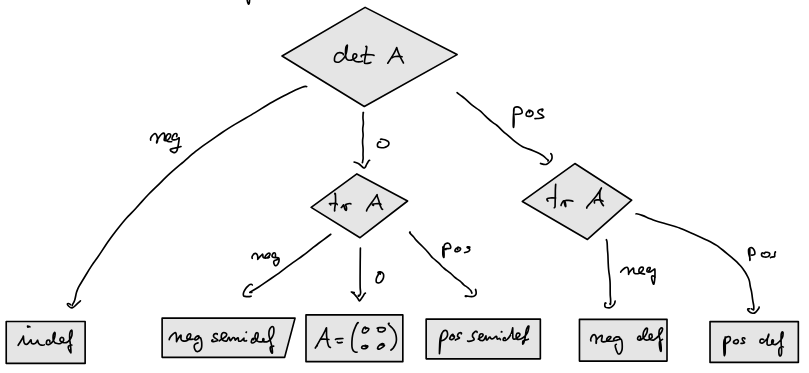
\includegraphics[width=\linewidth]{./sources/entscheidungsbaum-definitheit.png}
    \end{minipage}
  \rmrk{3.8.8}{If someone wants to contribute this pls do Oo. (Sylvester
  Kriterium)}
\subsection{Umkehrsatz}
  \definition{3.10.0}{lokale umkehrbarkeit}
    $U\in R^n$ offen. $f:U\rightarrow\mathbb R^n$ heisst \textbf{lokal
    umkehrbar} bei $y\in U$ falls offene $V,W\subseteq\mathbb R^n$ existieren
    mit $y\in V, f(y)\in w$, sodass $f|_V:V\rightarrow W$ bijektiv ist.\\
    Bzw. es existiert $g:W\rightarrow V$ sodass $f|_V\circ g=id_W, g\circ
    f|_W=id_V$. $g$ ist die umkehrfunktion von $f|_V$\\
  \definition{3.10.2}{Satz der Umkehrfunktion}
  $U\in\mathbb R^n$ offen, $f:U\rightarrow\mathbb R^n, f\in C^k, k\geq1$ und
  $J_f(y)$ eine invertierbare Matrix, dann ist $f$ lokal umkehrbar bei y, die
  Umkehrfunktion $g$ ist $C^k$ und $$J_g(f(y))=(J_f(y))^{-1}$$

